\documentclass[titlepage, a4paper]{article}
\usepackage{hyperref}
\usepackage{graphicx}
\usepackage[utf8]{inputenc}
\usepackage[english]{babel}


\title{
	Quarto! Minimax player \\
	IT3105 \\
}
\author{
	Nordmoen, Jørgen H. \\
	Østensen, Trond
}

\date{\today}

\begin{document}
\pagenumbering{RomanType}
\maketitle

\begin{abstract}\label{abstract}
	This paper is an introduction to our Quarto! minimax player. In this we will try to
	explain how we created our implementation, what sort of decisions the player makes
	the reasoning behind it and our result both against other configurations of our player
	and against other students minimax implementations.
\end{abstract}

\newpage
\tableofcontents

\begin{figure}[htb]
	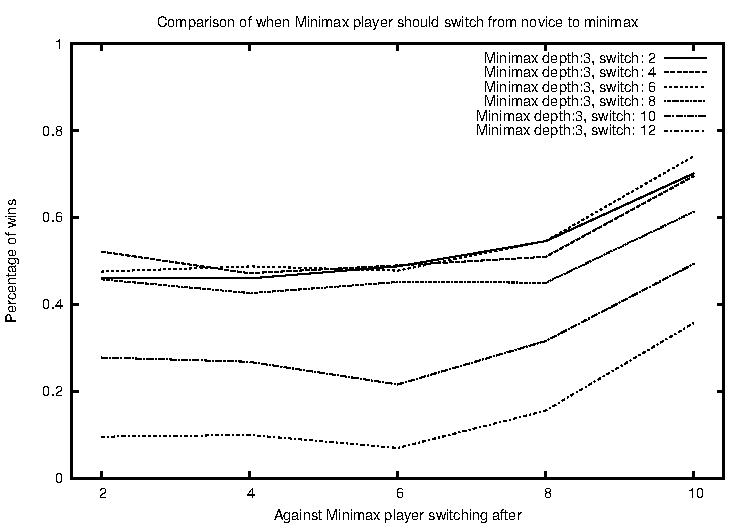
\includegraphics{graphs/switch.pdf}
	\label{fig:minimax switch}
	\caption{Graph describing our minimax switch results}
\end{figure}

\pagenumbering{arabic}

\end{document}
